%
% Slides for Networking Seminar - Spring 2017
% Author: Kirk Webb
%

% Document/preso setup stuff.
\documentclass[xcolor=pdftex,dvipsnames,table]{beamer}
\usepackage{alltt}
\usepackage{pdfpages}
\usetheme{CambridgeUS}
\usecolortheme{beaver}
\title{QuickC}
\subtitle{Practical sub-millisecond transport for small cells}
\setbeamercolor{subtitle}{fg=blue!80!black}
\setbeamerfont{subtitle}{shape=\itshape}
\author{Rakesh Misra et al.}
\institute{Stanford University}
\date{March 10, 2017}
\begin{document}

% Title page
\begin{frame}
\titlepage
\end{frame}

%%%
%%% Section
%%%
\section{Overview}

% Slide
\begin{frame}{What is this paper about?}
  \begin{itemize}
  \item Coordination between (small) mobile network cells.
  \item Motivation:
    \begin{itemize}
    \item Make it practical/easy to deploy small cells.
      \begin{itemize}
      \item Require only commodity internet link and power.
      \item Why deploy more small cells?
      \end{itemize}
    \item Cells transmitting on the same carrier need to minimize interference.
    \item Stale coordination data causes significant loss of efficiency.
    \end{itemize}
  \end{itemize}
\end{frame}

% Slide
\begin{frame}{What are the stated contributions?}
  \alert{\centerline{\emph{QuickC: low-latency underlay coordination channel for cells.}}}
  \vspace{2mm}
  \begin{itemize}
  \item QuickC channel operates concurrently with regular LTE (same freq).
  \item End-to-end latency of $<$ 1ms (vs. 20ms for regular LTE RAN).
  \item Plug-and-play design/implementation: No invasive changes.
  \item Implemented using off-the-shelf components.
  \item Minimally disruptive to co-channel LTE RAN traffic.
  \end{itemize}
\end{frame}

%%
%% Section
%%
\section{Details}

% Slide
\begin{frame}{The 1ms barrier}
  \setbeamercovered{invisible}
  \only<1>{\centerline{1 ms? Really?}}
  \only<2>{\centerline{\huge{Really.}}}
  \only<3>{\centerline{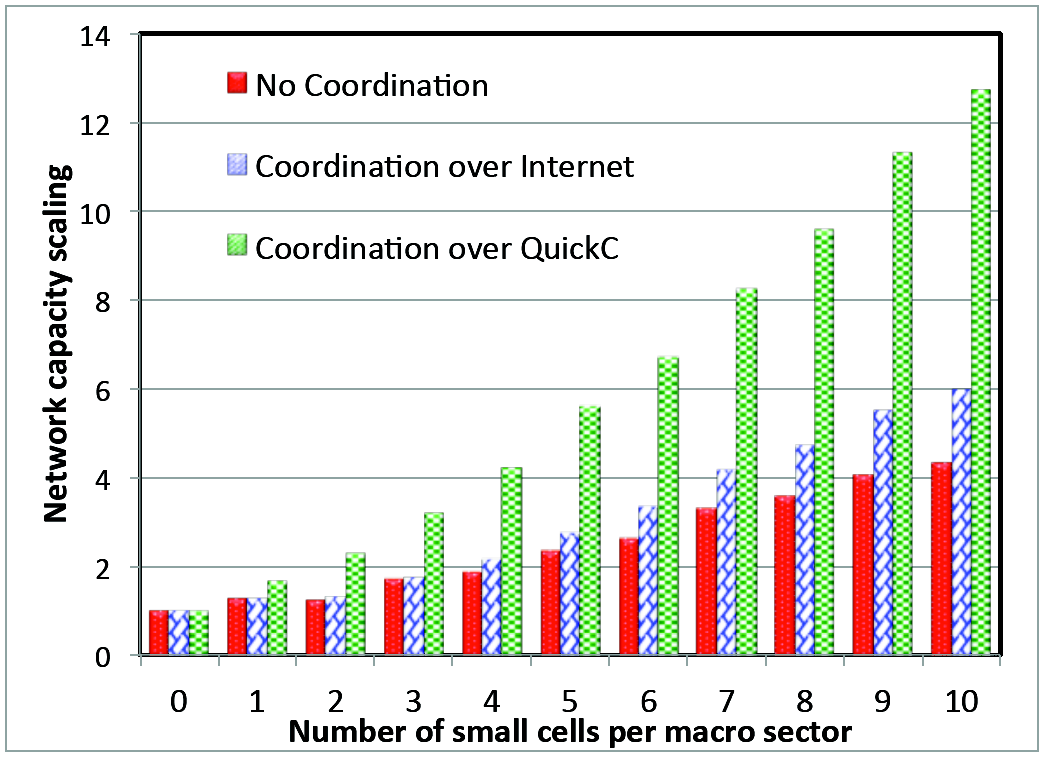
\includegraphics[width=0.8\textwidth]{./figs/quickc-comparison.png}}}
\end{frame}

% Slide
\begin{frame}{The 1ms barrier, cont'd}
  \begin{itemize}
  \item Coordinated MultiPoint Joint Transmission (CoMP-JT) needs tight coordination.
  \item ``Precoding vectors'' (MIMO-ish) become sub-optimal with stale data.
  \item Interference coherence times and traffic bursts: $~1ms$.
    \begin{itemize}
    \item Client channel to any one cell ``decorrelates'' significantly in 4-5ms.
    \item LTE client SINR changes in 1-2ms.
    \end{itemize}
  \end{itemize}
\end{frame}

% Slide
\begin{frame}{The 1ms barrier, cont'd II}
  \begin{itemize}
  \item Last mile commodity Internet latency (one-way) is typically $>14ms$.
  \item Throughput is generally sufficient for a small cell ($>50Mbps$).
  \item Dedicated front-haul to small cells impractical (expensive).
  \end{itemize}
\end{frame}

% Slide
\begin{frame}{QuickC Design}
  \begin{itemize}
  \item Latency insensitive data traffic goes over commodity uplink.
  \item Send inter-cell control traffic (X2) over the air.
  \item Re-use operator's sub-1GHz band; \emph{\bf send as RF underlay}.
    \begin{itemize}
    \item Takes advantage of already-deployed infrastructure.
    \item Additional BBU+radio and directional antenna at small cell.
    \item Piggyback on CPRI uplink to radio unit at macro cell.
    \end{itemize}
  \item Custom encoding overlayed on regular LTE resource blocks.
    \begin{itemize}
    \item Just acting as a regular macro-cell client is too costly.
    \end{itemize}
  \end{itemize}
\end{frame}

% Slide
\begin{frame}{QuickC System Block Diagram}
  \centerline{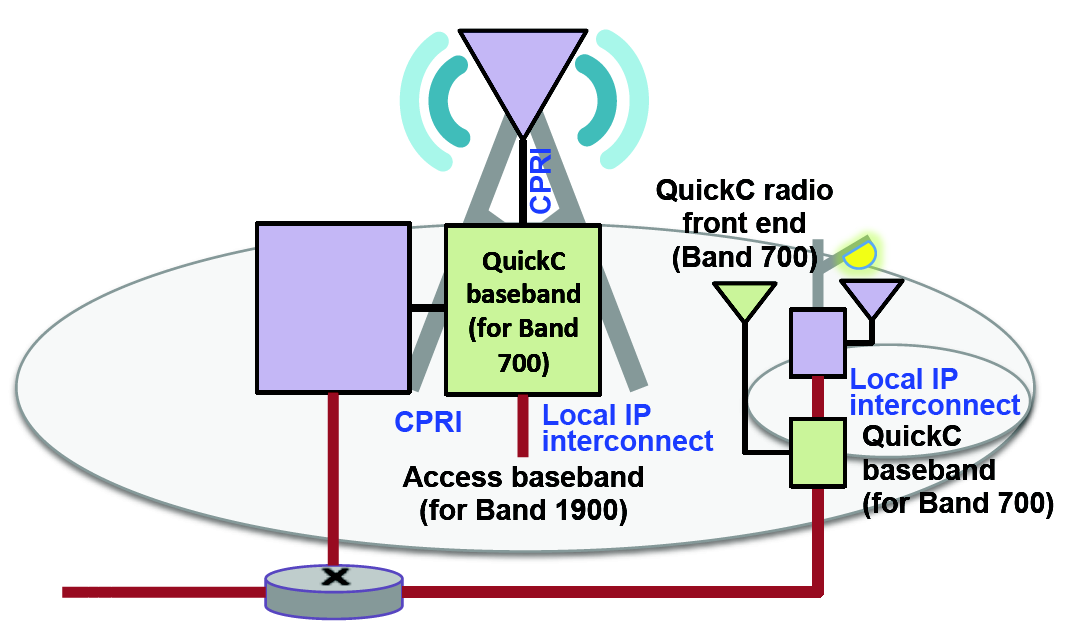
\includegraphics[width=\textwidth]{./figs/quickc-blockdiagram.png}}
\end{frame}

% Slide
\begin{frame}{QuickC Macro Cell BBU Block Diagram}
  \centerline{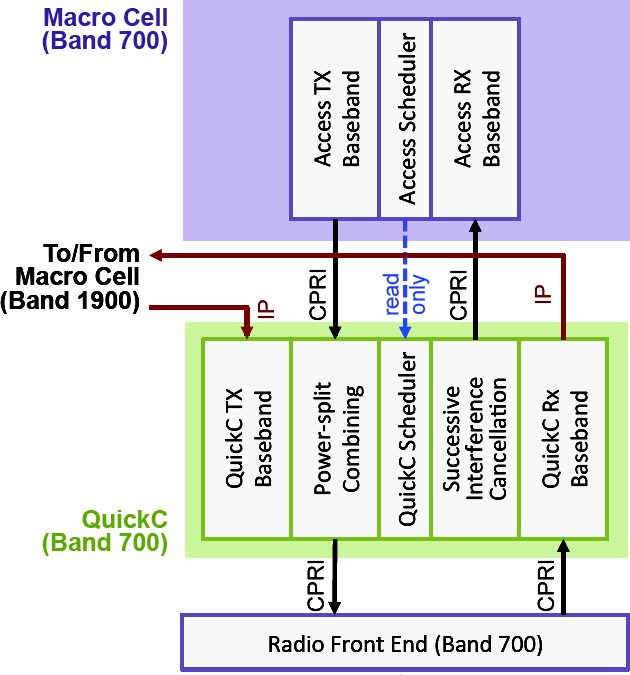
\includegraphics[width=0.55\textwidth]{./figs/quickc-macrodiagram.png}}
\end{frame}

% Slide
%\begin{frame}{QuickC Design Goals}
%  \begin{itemize}
%  \item Sub-millisecond latency and up to 4MBps bandwidth.
%  \item Low impact on regular network access (low single-digit percentage).
%  \item Modular add-on to existing cellular deployments.
%  \end{itemize}
%\end{frame}

% Slide
\begin{frame}{QuickC RF Underlay}
  \begin{itemize}
  \item Uses successive interference cancelation (SIC) technique.
    \begin{itemize}
    \item Xmit at significantly different power level vs. LTE.
    \item Cancel signal that is not at the power level you care about.
    \item Lower power from macro $=>$ small (in noise for normal LTE).
    \item Higher power from small $=>$ macro (directed signal).
    \end{itemize}
  \end{itemize}
\end{frame}

% Slide
\begin{frame}{QuickC Underlay Diagram}
  \centerline{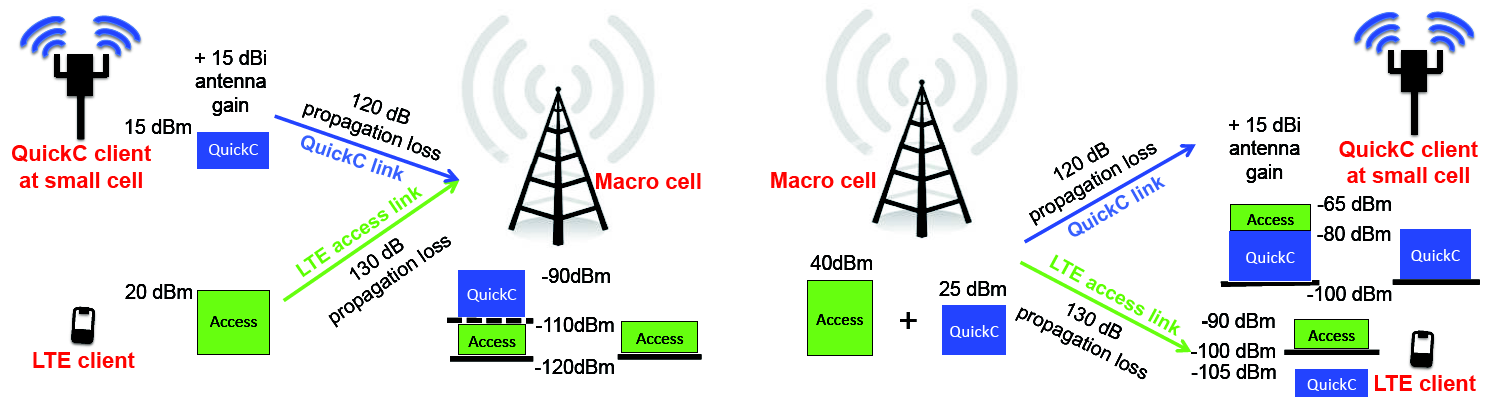
\includegraphics[width=\textwidth]{./figs/quickc-underlay.png}}
\end{frame}

\begin{frame}{Underlay Challenges}
  \begin{itemize}
  \item Cannot use standard LTE encoding on downlink (too coarse).
  \item Must schedule power levels based on LTE client SINR (whiteboard).
  \item Must carefully schedule uplink to avoid macro neighbor interference.
  \end{itemize}
\end{frame}

% Slide
\begin{frame}{QuickC channel interface}
  \centerline{\alert{\bf Uses clever tricks to meet $1ms$ budget}}
  \vspace{2mm}
  \begin{itemize}
  \item Encodes/decodes on a per-encoding (OFDM) symbol basis ($71.4{\mu}s$)
  \item RF resource blocks are pre-allocated for init at the macro cell.
  \item Exhibits same reliability as regular LTE due to same coding scheme.
  \item Uses ``noisy symbol'' forwarding for multihop transmission.
  \end{itemize}
\end{frame}

% Slide
\begin{frame}{QuickC Prototype Block Diagram}
  \centerline{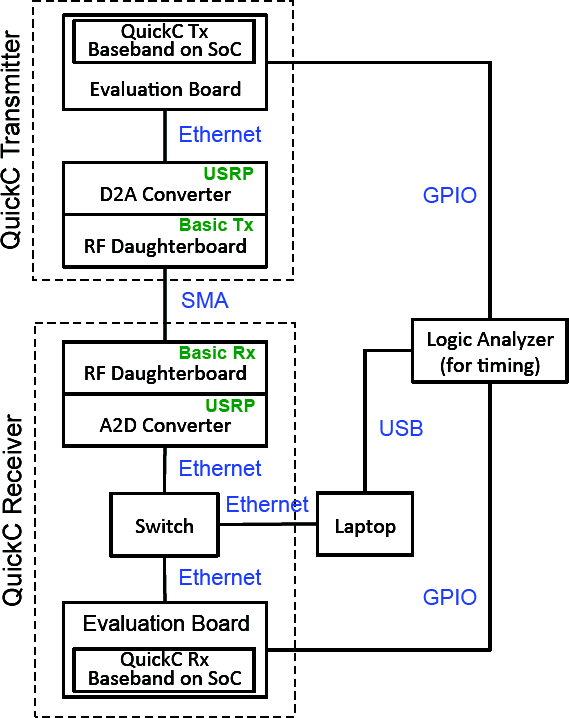
\includegraphics[width=0.48\textwidth]{./figs/quickc-prototype.png}}
\end{frame}

% Slide
\begin{frame}{Evaluation}
  \begin{itemize}
  \item Simulation and logic analyzer show prototype meets 1ms budget.
    \begin{itemize}
    \item $574{\mu}s$ small $<==>$ macro.
    \item $964{\mu}s$ small $<==>$ macro $<==>$ small.
    \item Low variability across repeated runs (within $2{\mu}s$).
    \end{itemize}
  \item Simluation indicates QuickC has low impact in LTE deployment.
    \begin{itemize}
    \item Simulated over 19 macro cells with 4 small cells per sector.
    \item Low degredation to neighbor cells (1.1dB median).
    \item Prototype shows similar degredation vs. channel emulator.
    \end{itemize}
  \end{itemize}
\end{frame}

%%%
%%% Section
%%%
\section{Discussion}

% Slide
\begin{frame}{Discussion items}
  \begin{itemize}
  \item Does all X2 traffic need to go over the QuickC underlay?
  \onslide<2->
  \item Uplink throughput does not fare as well at the 90th percentile.
  \onslide<3->
  \item Not needed for ``densification'' along corridors (roads, etc.).
  \onslide<4->
  \item Lessons for next-gen (*G) RAN?
  \end{itemize}
\end{frame}

% Slide
\begin{frame}{Blank}
  \large{\centerline{This page intentionally left blank...}}
\end{frame}

\end{document}

%%%%%%%%%%%%%%%%%%%%%%%%%%%%%%%%%%%%%%%%%%%%%%%%%%%%%%%%%%%%%%%%%%%%%%%%%%%%%%



